{\def\LTcaptype{none} % do not increment counter
\begin{longtable}[]{@{}
  >{\raggedright\arraybackslash}p{(\linewidth - 2\tabcolsep) * \real{0.1358}}
  >{\raggedright\arraybackslash}p{(\linewidth - 2\tabcolsep) * \real{0.8312}}@{}}
\toprule\noalign{}
\endhead
\bottomrule\noalign{}
\endlastfoot
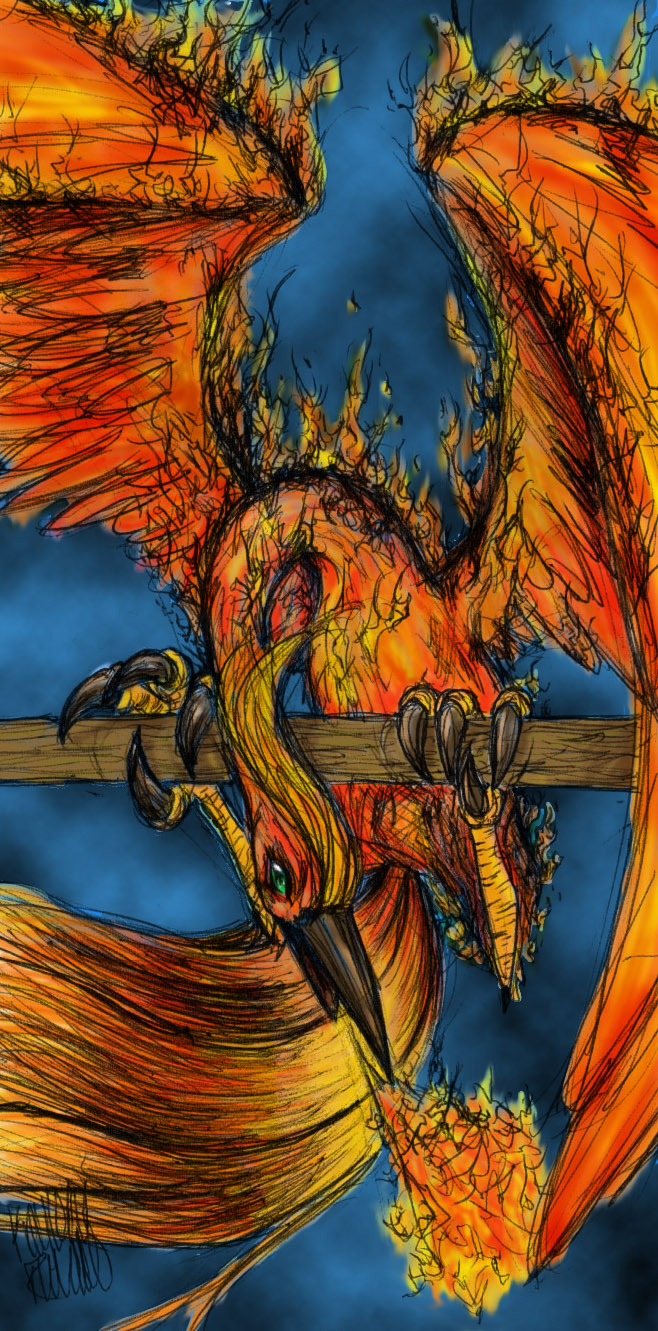
\includegraphics[width=3.35333in,height=9.8066in,alt={M:\textbackslash My Pictures\textbackslash Drawing Scans\textbackslash pheonixcoloured.JPG}]{./images/media/image1.jpeg} & \begin{minipage}[t]{\linewidth}\raggedright
\begin{quote}
\emph{\textbf{XDD}}

\emph{\textbf{User Guide}}
\end{quote}
\end{minipage} \\
\end{longtable}
}

\begin{quote}
Version 7.0.0.rc21-1

April 2012

I/O Performance, Inc.

Copyright © 1992-2012, I/O Performance, Inc.
\end{quote}

{\def\LTcaptype{none} % do not increment counter
\begin{longtable}[]{@{}
  >{\raggedright\arraybackslash}p{(\linewidth - 4\tabcolsep) * \real{0.2433}}
  >{\raggedright\arraybackslash}p{(\linewidth - 4\tabcolsep) * \real{0.0268}}
  >{\raggedright\arraybackslash}p{(\linewidth - 4\tabcolsep) * \real{0.3668}}@{}}
\toprule\noalign{}
\endhead
\bottomrule\noalign{}
\endlastfoot
\multicolumn{2}{@{}>{\raggedright\arraybackslash}p{(\linewidth - 4\tabcolsep) * \real{0.2702} + 2\tabcolsep}}{%
Principle Author:

Contributing Authors:} & Thomas M. Ruwart

\emph{tmruwart@ioperformance.com}

Steve Hodson, DoE/ORNL

\emph{hodsonsw@ornl.gov}

Steve Poole, DoE/ORNL

\emph{spoole@ornl.gov}

Bradly Settlemyer, DoE/ORNL

\emph{settlemyerbw@ornl.gov}

Russell Cattelan, Digital Elves

\emph{russell@thebarn.com}

Alex Elder \\
\multicolumn{2}{@{}>{\raggedright\arraybackslash}p{(\linewidth - 4\tabcolsep) * \real{0.2702} + 2\tabcolsep}}{%
} & \\
\multicolumn{2}{@{}>{\raggedright\arraybackslash}p{(\linewidth - 4\tabcolsep) * \real{0.2702} + 2\tabcolsep}}{%
Phone:} & 612-850-2918 \\
\multicolumn{2}{@{}>{\raggedright\arraybackslash}p{(\linewidth - 4\tabcolsep) * \real{0.2702} + 2\tabcolsep}}{%
Email:} & tmruwart@ioperformance.com \\
& \multicolumn{2}{>{\raggedright\arraybackslash}p{(\linewidth - 4\tabcolsep) * \real{0.3936} + 2\tabcolsep}@{}}{%
} \\
\end{longtable}
}

\textbf{Change History:}

The revision numbers have the following meaning. The ``number'' such as 5.7, 5.8, 5.9, \ldots etc. represent major release changes such as the addition of new options or sections to XDD.

{\def\LTcaptype{none} % do not increment counter
\begin{longtable}[]{@{}
  >{\raggedright\arraybackslash}p{(\linewidth - 6\tabcolsep) * \real{0.1701}}
  >{\raggedright\arraybackslash}p{(\linewidth - 6\tabcolsep) * \real{0.1612}}
  >{\raggedright\arraybackslash}p{(\linewidth - 6\tabcolsep) * \real{0.2091}}
  >{\raggedright\arraybackslash}p{(\linewidth - 6\tabcolsep) * \real{0.4232}}@{}}
\toprule\noalign{}
\endhead
\bottomrule\noalign{}
\endlastfoot
Revision & Date & Author & Description of Changes \\
7.0 & 18 JAN 2010 & Thomas M. Ruwart & Release of 7.0 \\
7.0 & 01FEB2011 & Thomas M. Ruwart & Pre-release 19 of 7.1 \\
7.0 & 07APR2011 & Thomas M. Ruwart & After release of Version 7.0 rc19 \\
7.0 & 18APR2011 & Thomas M. Ruwart & New heartbeat suboptions \\
7.0 rc21-1 & 02APR2012 & Thomas M. Ruwart & Maintenance Release \\
\end{longtable}
}

